\section{Testing}
\label{ch:testing}

This chapter documents the executed tests for the implemented system.
The testing evidence covers software correctness, user-interface
behavior, API integration, operational robustness, and the quality
boundary of the AI-assisted features. The executed validation includes
automated backend tests, automated frontend tests, screenshot-based UI
verification, API-level integration checks in Postman, manual workflow
tests, reliability-oriented backend tests, and AI-specific evaluation.

\subsection{Testing Strategy and Methodology}

The testing structure follows the architecture of the implemented
system. The backend contains route handlers, validation schemas,
persistence logic, RAG retrieval, OCR preprocessing, and provider
abstractions. The frontend contains page-level workflows for
authentication, recipe generation, recipe history, saved recipes, and
nutrition-label extraction. The executed tests are therefore grouped
into multiple layers with different goals.

\begin{itemize}
	\item \textbf{Unit and functional testing} validates backend route
	behavior, schema validation, service logic, and frontend rendering
	behavior under controlled conditions.
	\item \textbf{UI testing} verifies that the main user-facing pages are
	usable and display the expected workflow states.
	\item \textbf{Integration and end-to-end API testing} verifies that the
	HTTP layer, authentication flow, persistence layer, and paginated
	history endpoints work together correctly.
	\item \textbf{Advanced reliability testing} checks whether the backend
	remains stable under repeated requests and small mocked bursts without
	measuring uncontrollable external-provider latency.
\end{itemize}

Deterministic behavior such as authentication and history scoping is
validated with automated assertions. User-visible workflow states are
documented through rendered pages and screenshots. Integration behavior
is validated through HTTP requests in Postman. Reliability checks use
mocked provider dependencies so that the observed results reflect local
system behavior rather than external service latency.

Coverage was used as a supporting indicator together with functional
evidence. The backend focus was the public route groups,
authentication guards, persistence flows, schema validation, OCR
preprocessing, and RAG support logic. The frontend focus was the main
pages and their most important guest and authenticated branches.

\subsection{Unit and Functional Testing}

\subsubsection{Backend automated test suite}

The backend test suite was executed with \texttt{pytest} against the
FastAPI application and its supporting modules. The tests cover
authentication, protected-route behavior, recipe generation endpoints,
OCR persistence endpoints, schema validation, service-provider
selection, RAG retrieval logic, image preprocessing, rate limiting, and
mocked reliability scenarios. The executed suite therefore covers both
internal helper logic and the request/response contracts exposed by the
backend to the frontend.

The backend suite completed successfully with \textbf{46 passing tests}.
The terminal output is shown in Figure~\ref{fig:pytest-suite}.

\begin{figure}[H]
	\centering
	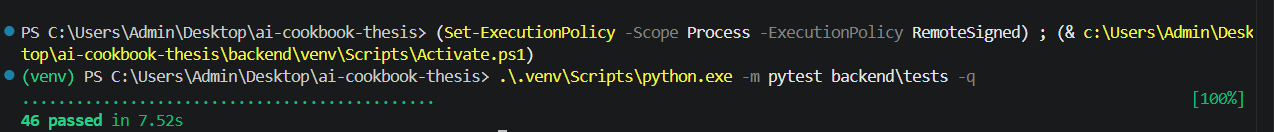
\includegraphics[width=0.9\textwidth]{images/PytestScreenshot.png}
	\caption{Successful backend automated test execution with \texttt{pytest}}
	\label{fig:pytest-suite}
\end{figure}

The executed backend tests are concentrated in four areas:

\begin{itemize}
	\item \textbf{Authentication and authorization:} signup, login, token
	validation, invalid-token rejection, expired-token rejection, and
	protected-route access control.
	\item \textbf{Persistence and user scoping:} saving generated recipes,
	listing recipe history, saving OCR extractions, and ensuring that one
	user cannot see another user's saved content.
	\item \textbf{Validation and preprocessing:} request-schema cleaning,
	image-type checks, image-size limits, and OCR preprocessing rules.
	\item \textbf{Retrieval and orchestration logic:} ingredient conflict
	detection, preference conflict detection, retrieval query formation,
	candidate ranking behavior, and provider selection.
\end{itemize}

The backend evidence covers security, persistence, and intermediate
business logic in addition to basic route responses.

\subsubsection{Frontend automated functional tests}

The frontend test suite was executed with \texttt{Vitest} and the
\texttt{jsdom} environment. These tests validate the behavior of the
React pages and components, including form handling, conditional
rendering, authenticated page states, and structured result display.

The frontend suite completed successfully with \textbf{12 passing tests
across 6 test files}, as shown in
Figure~\ref{fig:vitest-suite}. The tested areas include the login page,
generate-recipe page, saved-recipes page, recipe-history page,
nutrition-label page, and the shared nutrition-grid component.

\begin{figure}[H]
	\centering
	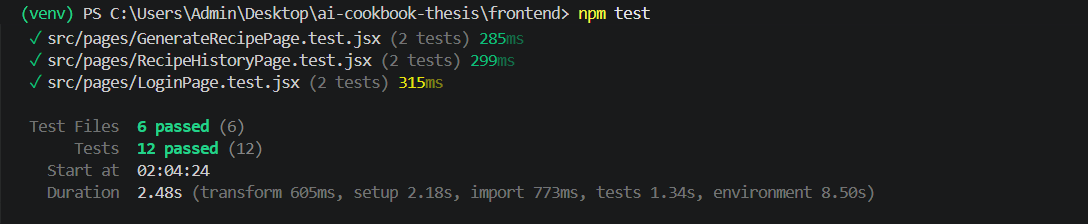
\includegraphics[width=0.9\textwidth]{images/VitestScreenshot.png}
	\caption{Successful frontend automated test execution with \texttt{Vitest}}
	\label{fig:vitest-suite}
\end{figure}

The frontend tests verify several behaviors that are visible to the end
user:

\begin{itemize}
	\item validation errors are shown when required fields are missing,
	\item saved profile defaults are reused correctly during recipe
	generation,
	\item login and profile-update requests are sent with the expected
	payloads,
	\item protected pages display correct guest-only guidance when the user
	is not authenticated,
	\item history entries can be rendered and expanded correctly,
	\item nutrition data is rendered consistently in both recipe and OCR
	contexts.
\end{itemize}

The backend and frontend automated suites provide the main
deterministic correctness evidence for the application.

\subsubsection{Measured test coverage}

In addition to counting passing tests, the executed suites were also
measured for implementation coverage. Backend coverage was measured with
\texttt{coverage.py} over the \texttt{pytest} run, while frontend
coverage was measured with the \texttt{Vitest} V8 coverage provider.
Table~\ref{tab:coverage-summary} summarizes the resulting indicators.

\begin{table}[H]
	\centering
	\small
	\renewcommand{\arraystretch}{1.2}
	\begin{tabularx}{\textwidth}{|p{2.3cm}|p{2.4cm}|p{2.5cm}|>{\raggedright\arraybackslash}X|}
		\hline
		\textbf{Layer} & \textbf{Tool} & \textbf{Metric} & \textbf{Result} \\
		\hline
		Backend & \texttt{coverage.py} + \texttt{pytest} & Statement coverage & \textbf{77\%} overall (1138 of 1474 statements executed). \\
		\hline
		Frontend & \texttt{Vitest} V8 coverage & Statement / line coverage & \textbf{72.98\%} statements and \textbf{74.90\%} lines. \\
		\hline
		Frontend & \texttt{Vitest} V8 coverage & Branch / function coverage & \textbf{55.18\%} branches and \textbf{64.93\%} functions. \\
		\hline
		\end{tabularx}
	\caption{Coverage indicators measured for the automated test suites}
	\label{tab:coverage-summary}
\end{table}

These percentages should be interpreted together with the covered
modules. The backend coverage is strongest in the directly relevant
application layers: \texttt{main.py} reached 100\%, route modules such
as \texttt{auth.py}, \texttt{ocr.py}, and \texttt{recipes.py} reached
98\%, 97\%, and 94\%, \texttt{schemas.py} reached 98\%, and
\texttt{rag\_service.py} reached 91\%. The lower backend totals are
mainly caused by thin provider-adapter and externally dependent modules
such as \texttt{llm\_service.py}, \texttt{ocr\_google\_vision\_provider.py},
\texttt{recipe\_image\_service.py}, and \texttt{vector\_store\_service.py},
which are harder to execute comprehensively in a deterministic local
test environment without turning the thesis suite into a network-
dependent integration harness.

The frontend coverage similarly reflects the actual design of the
application. The most important page-level flows are exercised, but some
secondary branches, especially inside the saved-recipes page, remain
less covered because the current suite prioritizes core navigation,
validation, authenticated state handling, and result rendering over
exhaustive UI edge-case permutation.

\subsubsection{Representative executed test cases}

Table~\ref{tab:representative-test-cases} presents a representative
selection of executed test cases, including the test steps, expected
result, and observed result.

\begin{table}[H]
	\centering
	\scriptsize
	\renewcommand{\arraystretch}{1.2}
	\begin{tabularx}{\textwidth}{|>{\raggedright\arraybackslash}p{1.6cm}|>{\raggedright\arraybackslash}p{2.4cm}|>{\raggedright\arraybackslash}X|>{\raggedright\arraybackslash}X|>{\raggedright\arraybackslash}X|}
		\hline
		\textbf{Layer} & \textbf{Case} & \textbf{Test Steps} & \textbf{Expected Result} & \textbf{Observed Result} \\
		\hline
		Frontend automated & Empty recipe submission validation & Open the Generate page, leave the ingredient field empty, and press \texttt{Generate Recipe}. & A validation error is shown and no API request is sent. & The executed \texttt{Vitest} case rendered the message ``Please enter at least one ingredient'' and confirmed that the mocked API function was not called. \\
		\hline
		Backend automated & Protected profile access without token & Send \texttt{GET /me} without an authorization header. & The endpoint rejects the request with \texttt{401 Unauthorized}. & The executed \texttt{pytest} case returned status code 401, confirming correct protected-route enforcement. \\
		\hline
		Backend automated & Authenticated recipe generation persists history & Generate a recipe as an authenticated user, then request \texttt{/recipes/history}. & The generated recipe is stored and later visible in history with the expected metadata. & The executed backend test verified one history item with the generated identifier, the expected title, and unsaved state metadata. \\
		\hline
		Frontend automated & Saved defaults reused during generation & Render the Generate page for a logged-in user with stored preferences and allergies, enter only ingredients, and submit. & The request payload automatically includes the saved defaults and the page renders a structured recipe response. & The executed \texttt{Vitest} case confirmed both the outgoing payload and the displayed recipe result. \\
		\hline
		Manual scenario & Successful login and account view & Open the Login page, submit valid credentials, and navigate to the Account page. & Authentication succeeds and profile information is displayed. & The executed manual run displayed the account page together with the saved dietary-preference and allergy sections. \\
		\hline
		Manual + OCR evaluation & OCR extraction on a clear nutrition label & Upload \texttt{nutrition-facts.jpg} and execute extraction on the Food Labels page. & Structured nutrition values and raw OCR text are returned without page failure. & The executed case returned calories 257, protein 8\,g, carbohydrates 39.8\,g, fat 9.4\,g, sugar 2.1\,g, sodium 41\,mg, fiber 10\,g, and readable raw OCR output. \\
		\hline
		\end{tabularx}
	\caption{Representative executed test cases with steps, expected result, and observed result}
	\label{tab:representative-test-cases}
\end{table}

\subsection{UI Testing}

\subsubsection{Purpose of screenshot-based UI verification}

Automated frontend tests confirm logic and rendering decisions, but
visual verification was also documented for the main user-facing
workflows. The application contains multiple screens where the
arrangement of controls, messages, cards, and structured outputs is
part of the observed result. Screenshot-based UI verification therefore
documents the implemented pages and the expected sequence of user
actions.

\subsubsection{Main workflow screens}

Figure~\ref{fig:ui-home-login} shows the home page and the
authentication screen. These screenshots document the entry point into
the main workflows and the dedicated authentication view for login and
sign-up.

\begin{figure}[H]
	\centering
	\begin{minipage}{0.48\textwidth}
		\centering
		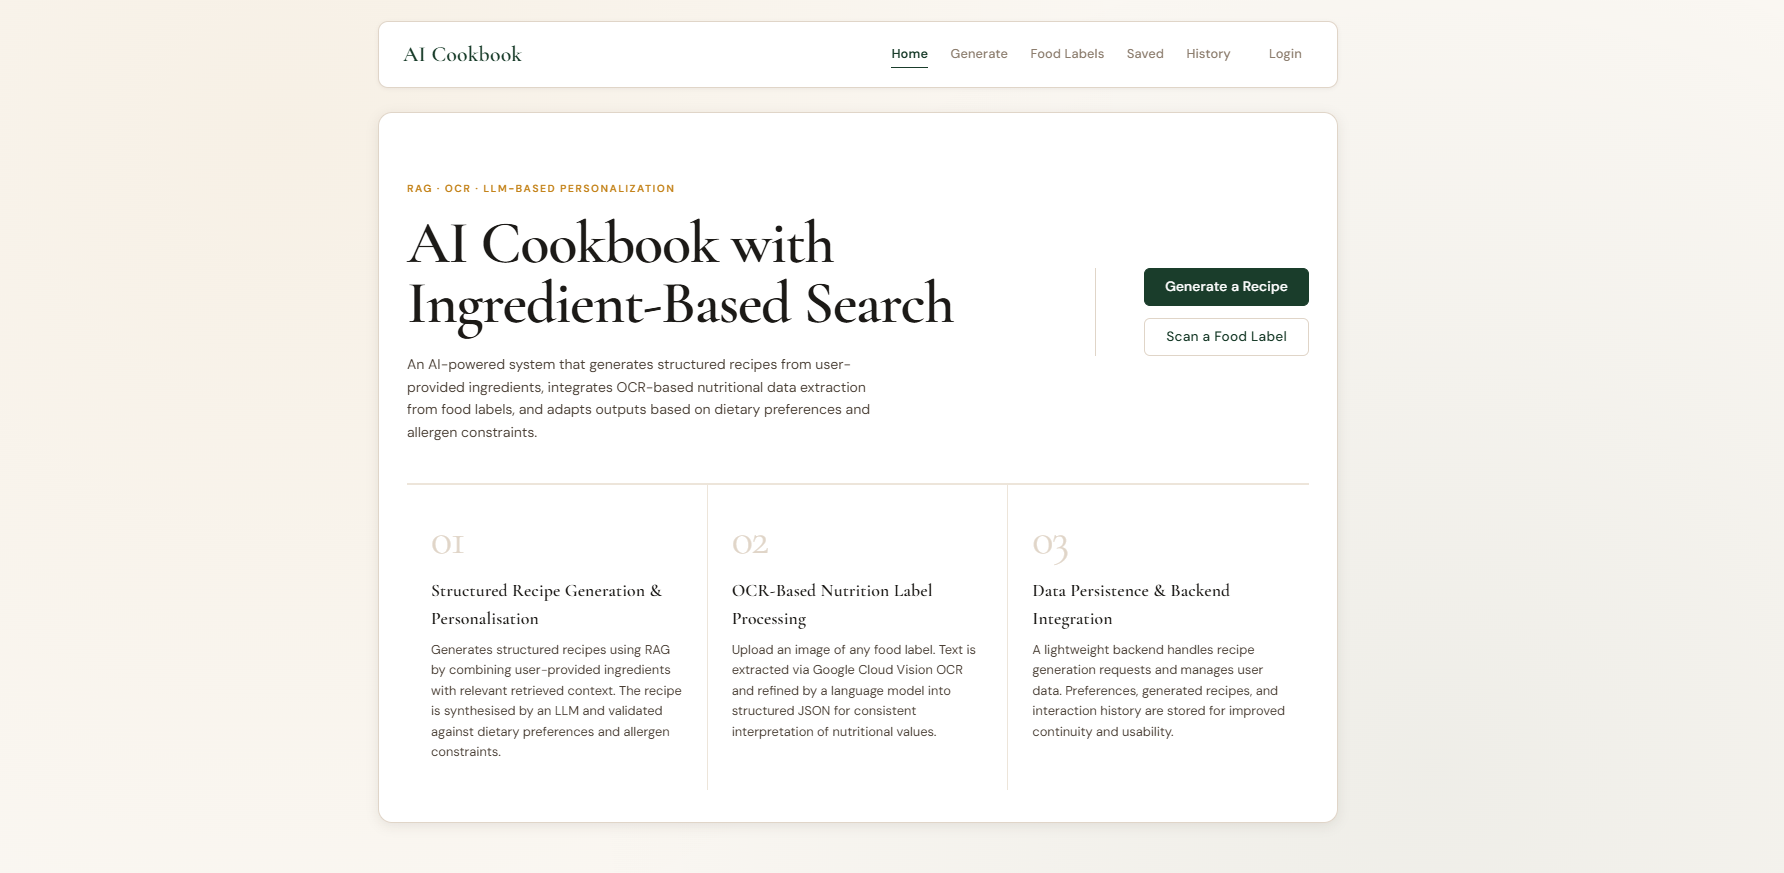
\includegraphics[width=\textwidth]{images/HomePage.png}
		\caption*{(a) Home page}
	\end{minipage}\hfill
	\begin{minipage}{0.48\textwidth}
		\centering
		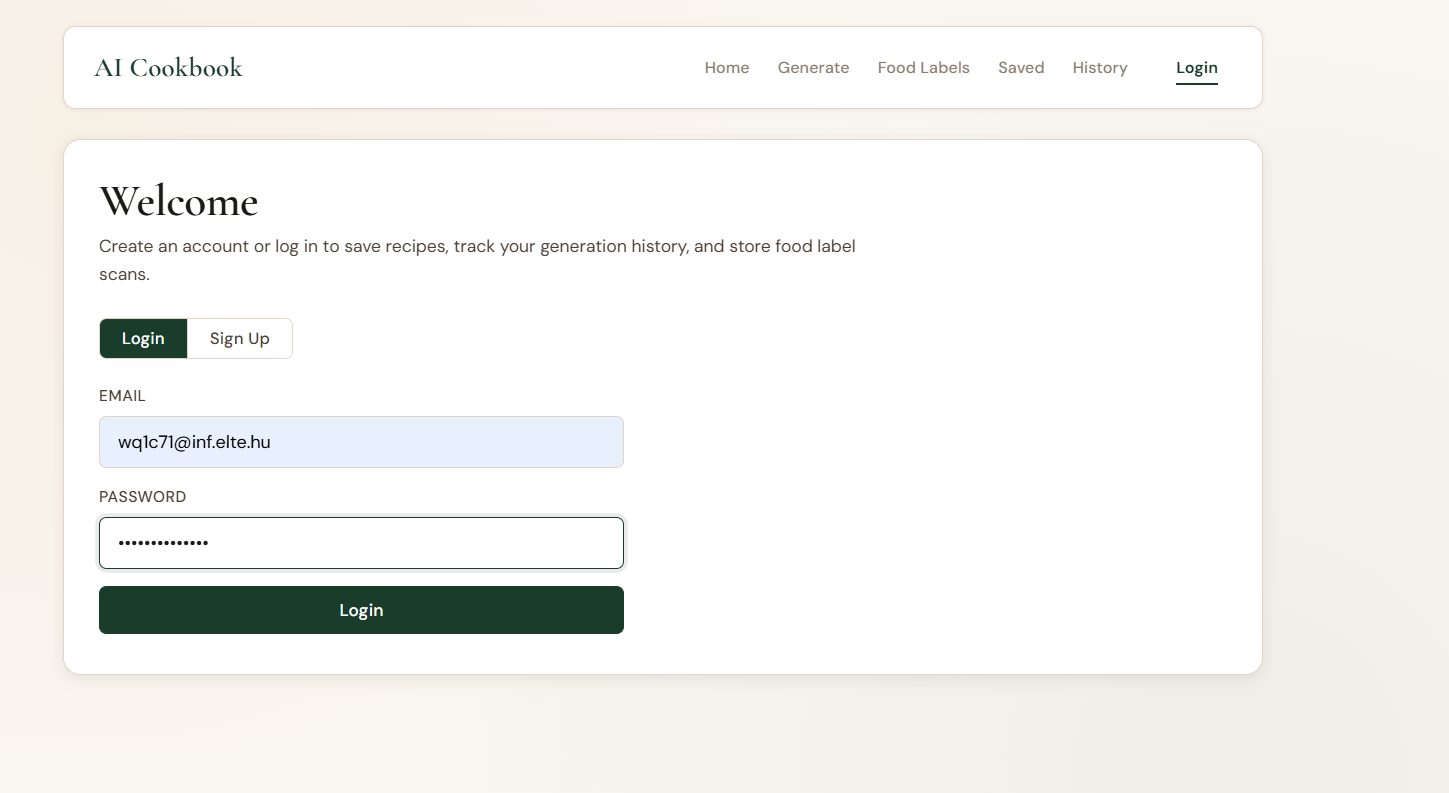
\includegraphics[width=\textwidth]{images/Login.png}
		\caption*{(b) Login and sign-up page}
	\end{minipage}
	\caption{Entry and authentication screens of the implemented frontend}
	\label{fig:ui-home-login}
\end{figure}

Figure~\ref{fig:ui-account-generate} shows the account page and the
recipe-generation page. The account page confirms that user defaults
for dietary preferences and allergies can be viewed and edited, while
the generate page confirms that ingredient input, structured output, and
recipe-specific response presentation are integrated into a single task
flow.

\begin{figure}[H]
	\centering
	\begin{minipage}{0.48\textwidth}
		\centering
		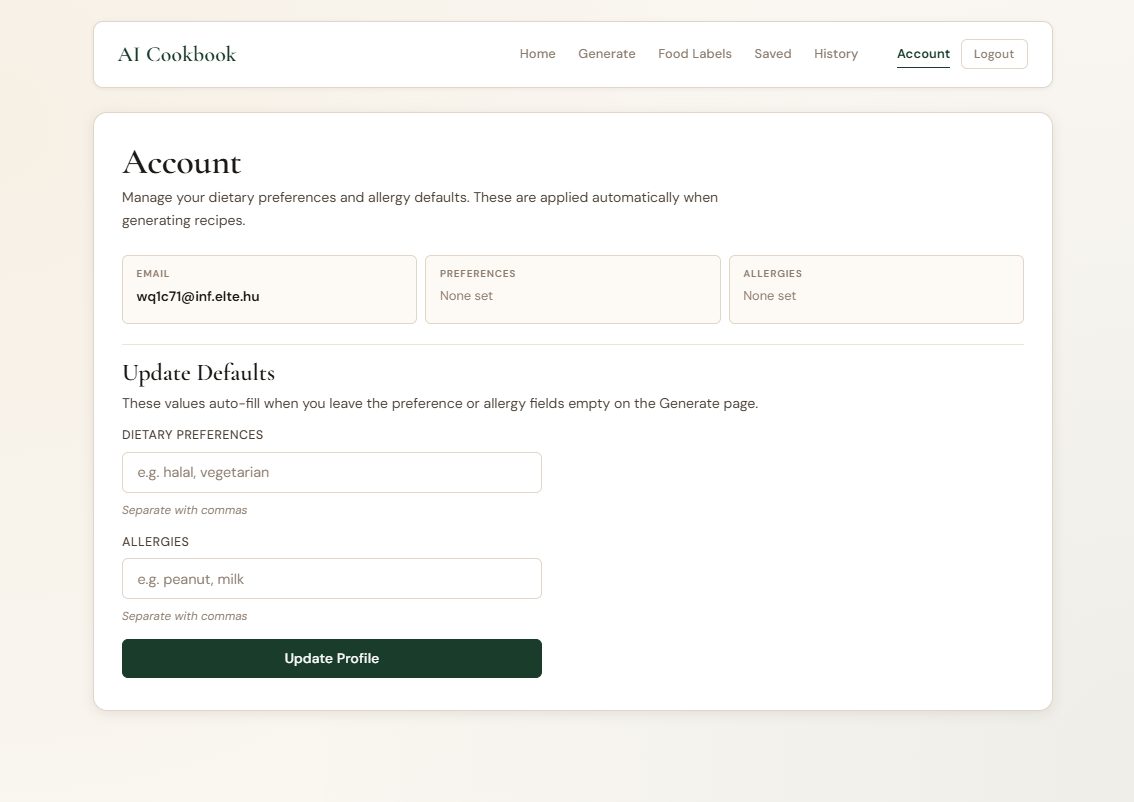
\includegraphics[width=\textwidth]{images/Account.png}
		\caption*{(a) Account and saved defaults}
	\end{minipage}\hfill
	\begin{minipage}{0.48\textwidth}
		\centering
		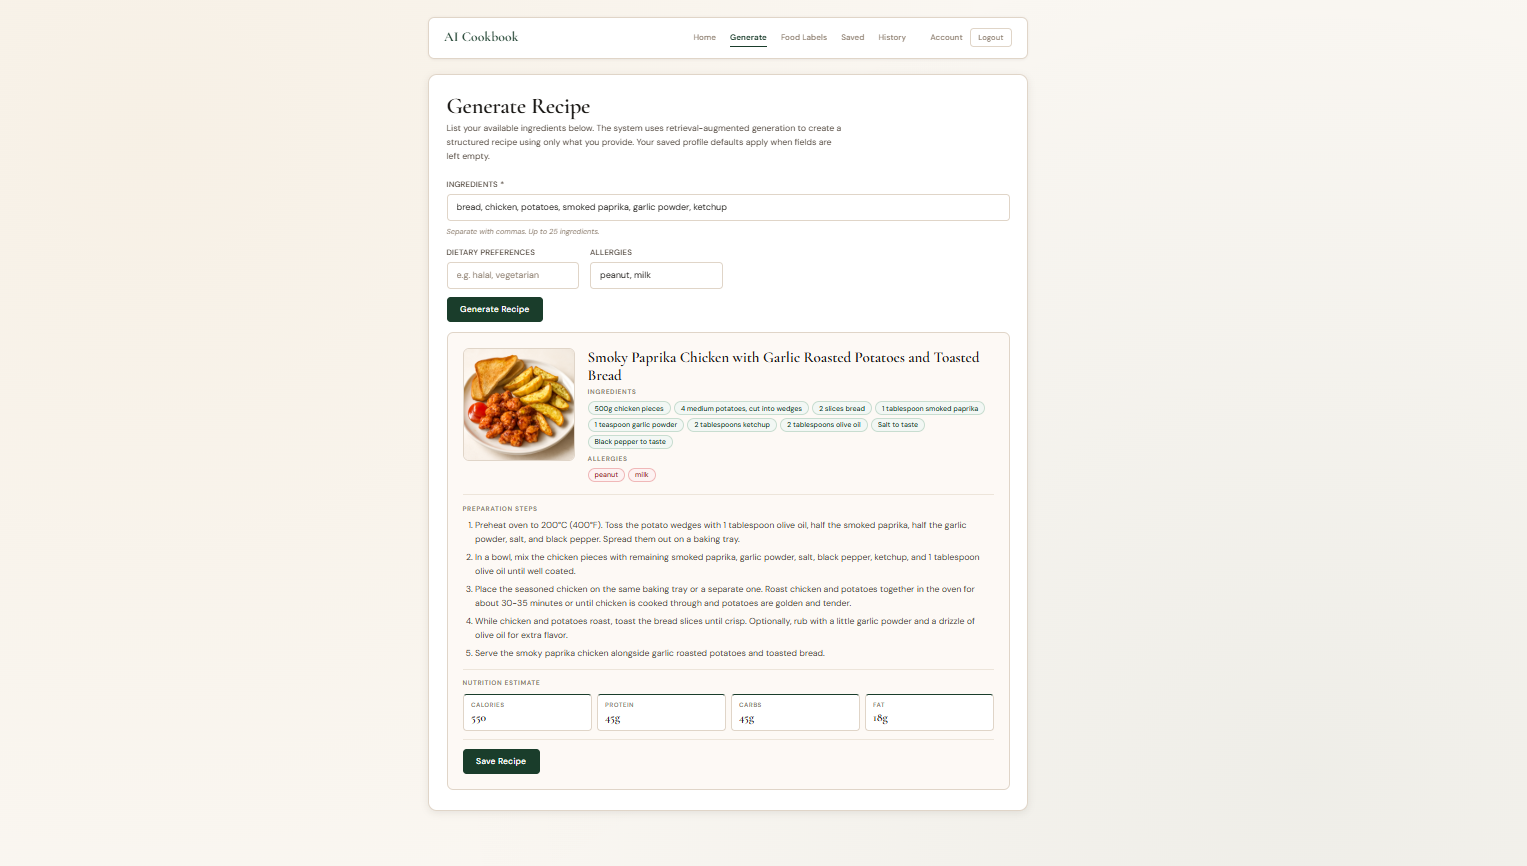
\includegraphics[width=\textwidth]{images/GenerateRecipe.png}
		\caption*{(b) Recipe generation workflow}
	\end{minipage}
	\caption{Authenticated profile management and recipe-generation UI}
	\label{fig:ui-account-generate}
\end{figure}

Figure~\ref{fig:ui-history-saved-ocr} shows the persistence-oriented
screens. These screenshots confirm that generated recipes, explicitly
saved recipes, and OCR nutrition-label processing all have dedicated
presentation flows in the interface.

\begin{figure}[H]
	\centering
	\begin{minipage}{0.32\textwidth}
		\centering
		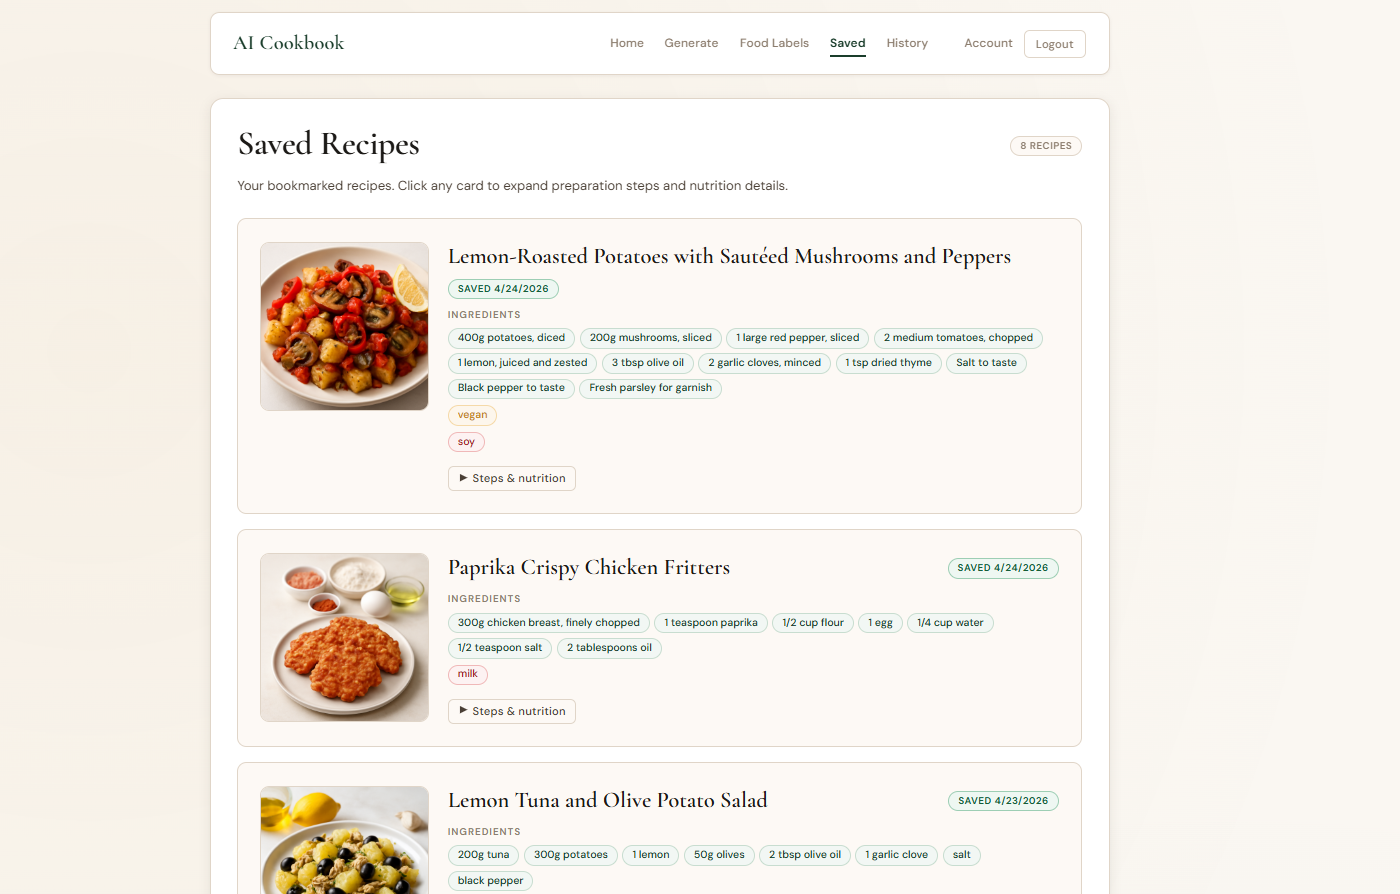
\includegraphics[width=\textwidth]{images/SavedRecipes.png}
		\caption*{(a) Saved recipes}
	\end{minipage}\hfill
	\begin{minipage}{0.32\textwidth}
		\centering
		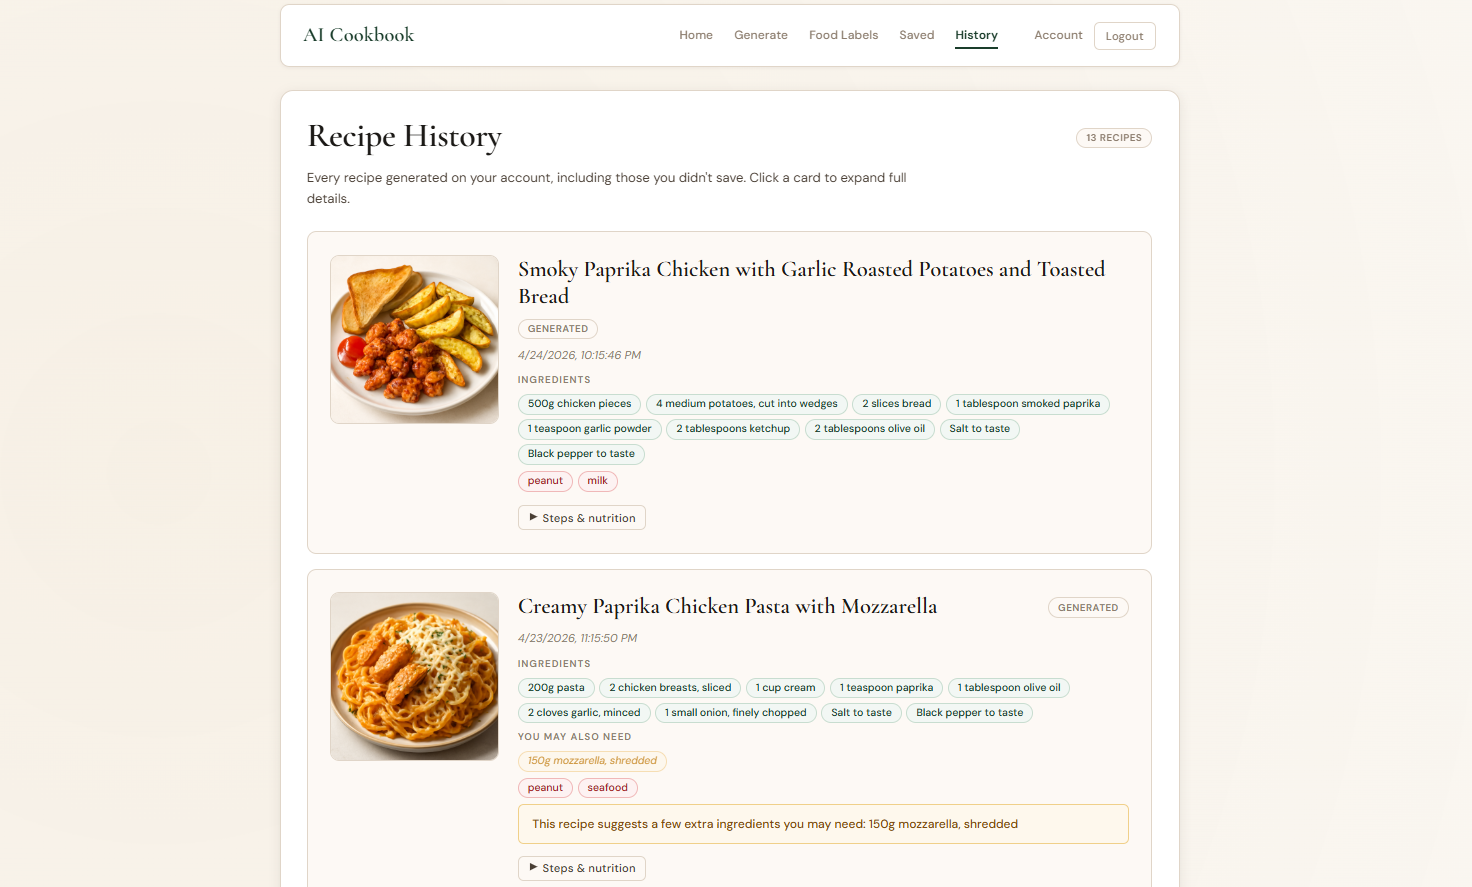
\includegraphics[width=\textwidth]{images/History.png}
		\caption*{(b) Recipe history}
	\end{minipage}\hfill
	\begin{minipage}{0.32\textwidth}
		\centering
		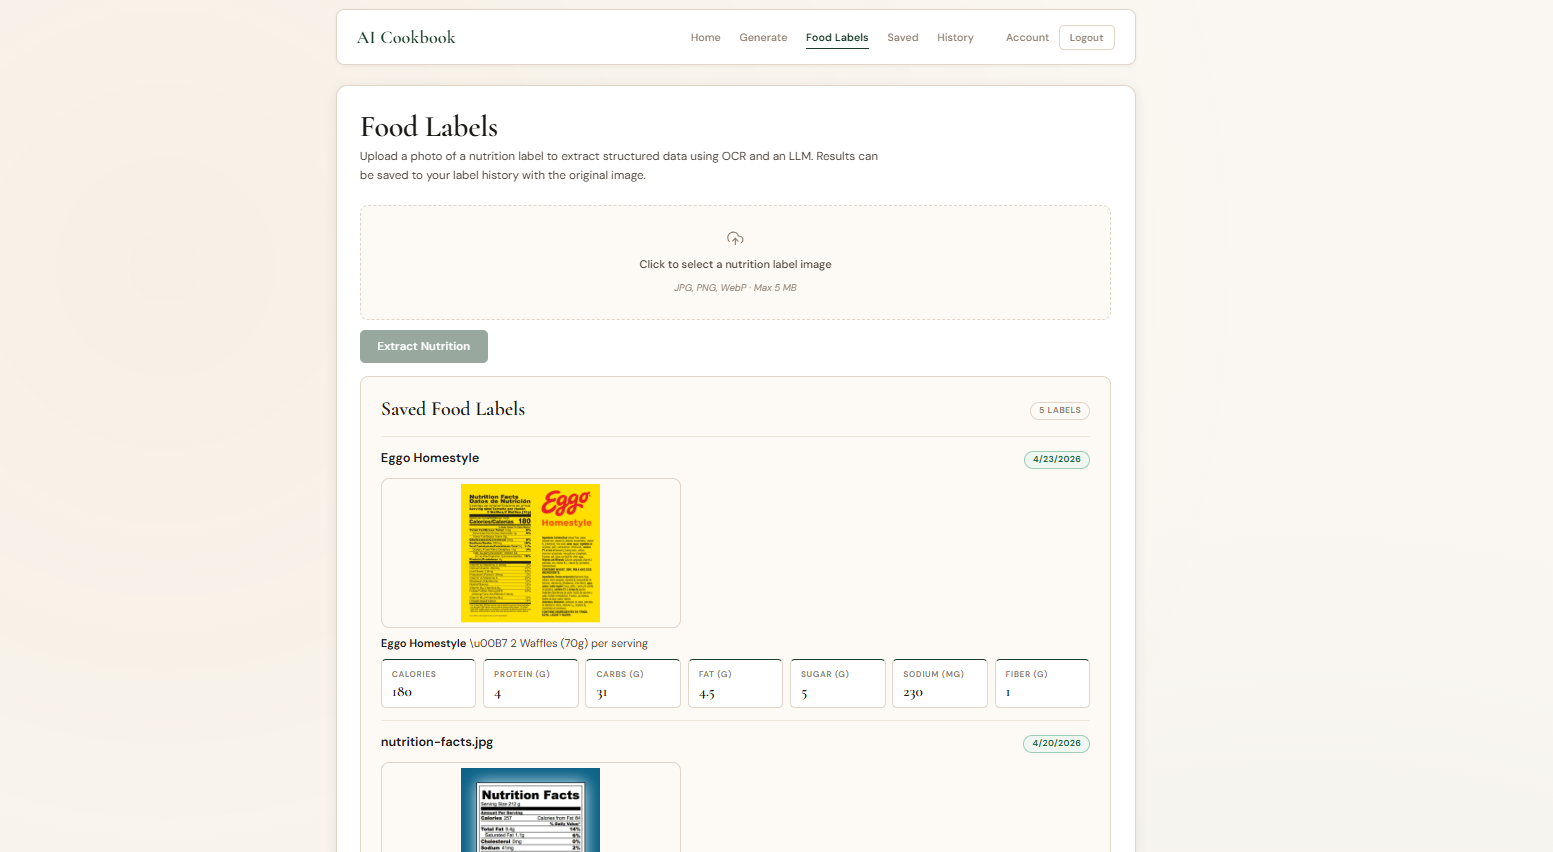
\includegraphics[width=\textwidth]{images/OCR.png}
		\caption*{(c) OCR nutrition-label workflow}
	\end{minipage}
	\caption{Persistence and OCR-related UI screens}
	\label{fig:ui-history-saved-ocr}
\end{figure}

These UI screenshots document three observed properties of the frontend:
the implemented workflows are present, guest and authenticated states
are separated clearly, and the outputs of recipe generation and OCR
extraction are presented in a readable task-oriented format.

\subsection{Integration and End-to-End Testing}

\subsubsection{Postman as API-integration evidence}

To validate the interaction between the HTTP layer, authentication,
backend persistence, and feature-specific routes, the project uses a
dedicated Postman collection. This collection provides request-level
evidence that the implemented API can be exercised outside the frontend
and behaves correctly through direct HTTP calls.

The collection itself is shown in
Figure~\ref{fig:postman-collection}. It documents that the API checks
were organized as a repeatable test set rather than as isolated ad hoc
requests.

\begin{figure}[H]
	\centering
	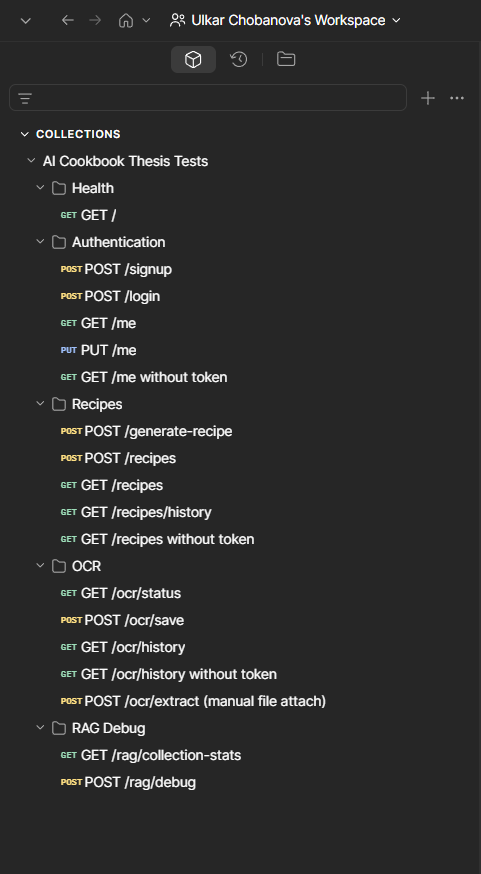
\includegraphics[width=0.82\textwidth]{images/POSTMAN/POSTMANcollection.png}
	\caption{Postman collection used for API-level integration testing}
	\label{fig:postman-collection}
\end{figure}

The Postman checks were executed in a sequence that follows the real
system lifecycle: health verification, account creation, login,
authenticated profile access, main feature calls, persistence actions,
and history retrieval. Figure~\ref{fig:postman-auth} shows the initial
health and authentication requests.

\begin{figure}[H]
	\centering
	\begin{minipage}{0.32\textwidth}
		\centering
		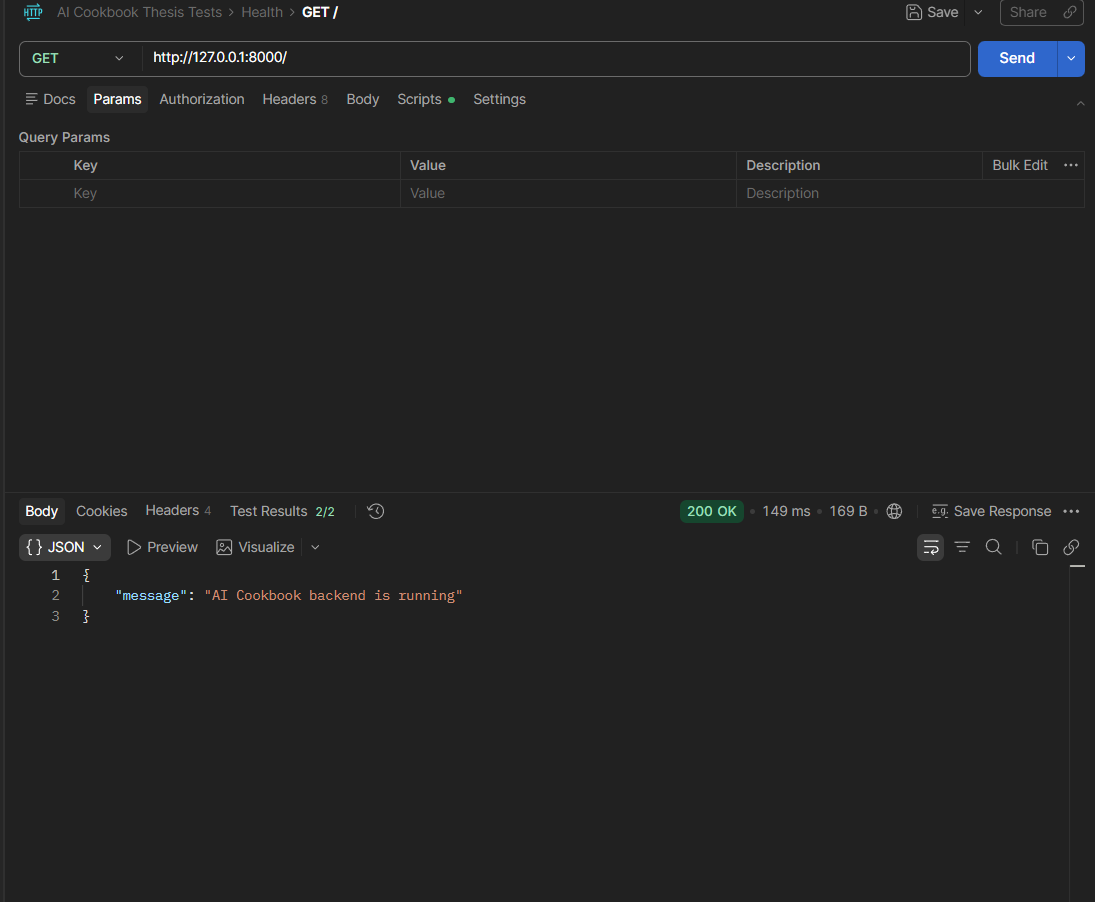
\includegraphics[width=\textwidth]{images/POSTMAN/POSTMANhealth.png}
		\caption*{(a) Health check}
	\end{minipage}\hfill
	\begin{minipage}{0.32\textwidth}
		\centering
		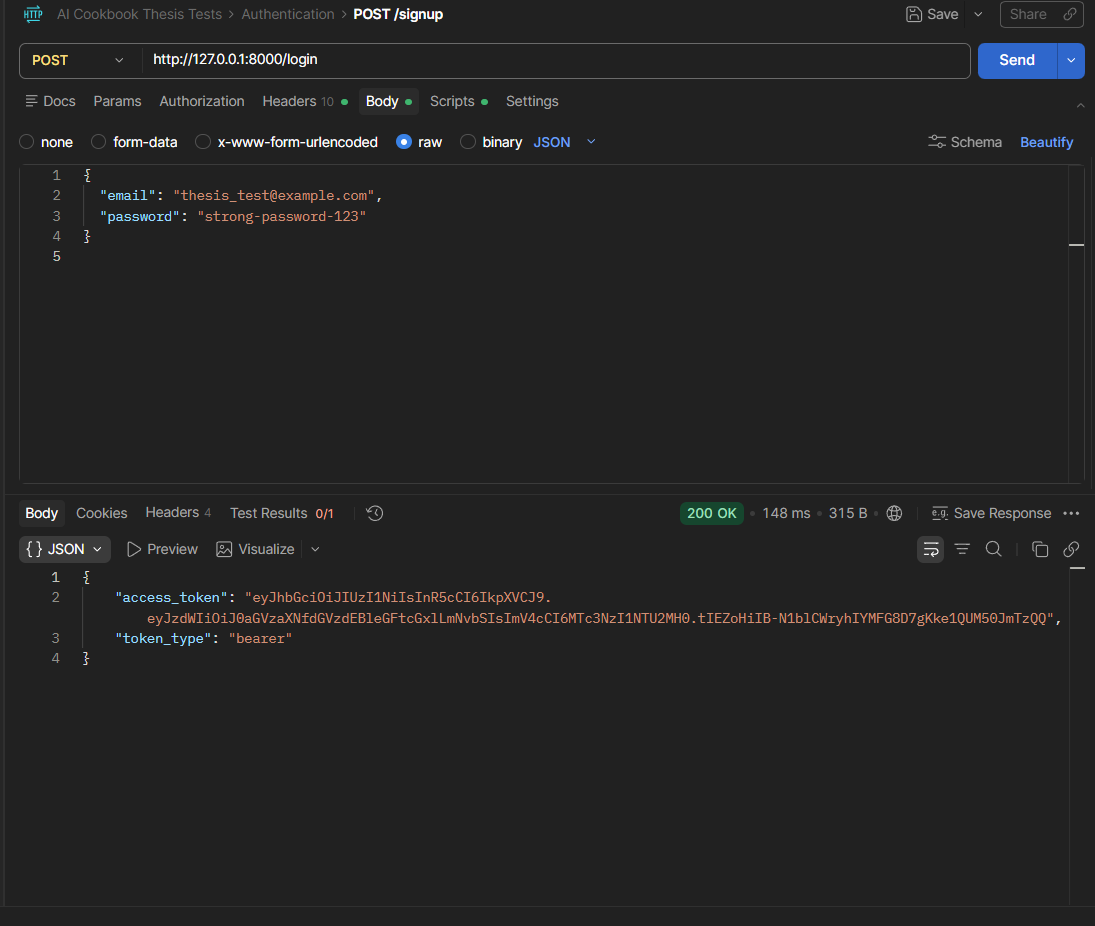
\includegraphics[width=\textwidth]{images/POSTMAN/POSTMANsignup.png}
		\caption*{(b) Signup request}
	\end{minipage}\hfill
	\begin{minipage}{0.32\textwidth}
		\centering
		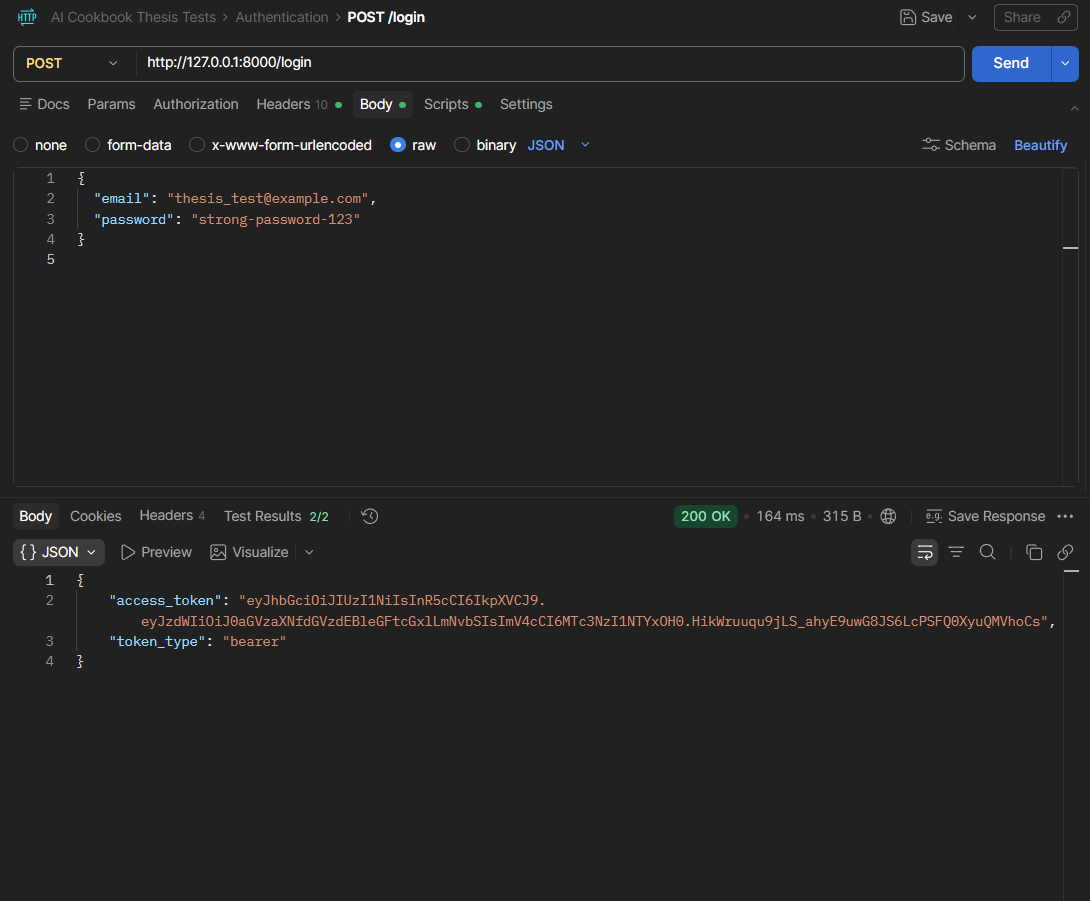
\includegraphics[width=\textwidth]{images/POSTMAN/POSTMANlogin.png}
		\caption*{(c) Login request}
	\end{minipage}
	\caption{Postman evidence for backend availability and authentication}
	\label{fig:postman-auth}
\end{figure}

The health-check response confirms that the backend is running and
reachable. The signup and login responses confirm that account creation
and token issuance work correctly through the public API boundary.

Figure~\ref{fig:postman-protected} shows the profile request and an
unauthorized access attempt. This pair documents both successful
authenticated access and rejection of unauthenticated access to
protected resources.

\begin{figure}[H]
	\centering
	\begin{minipage}{0.48\textwidth}
		\centering
		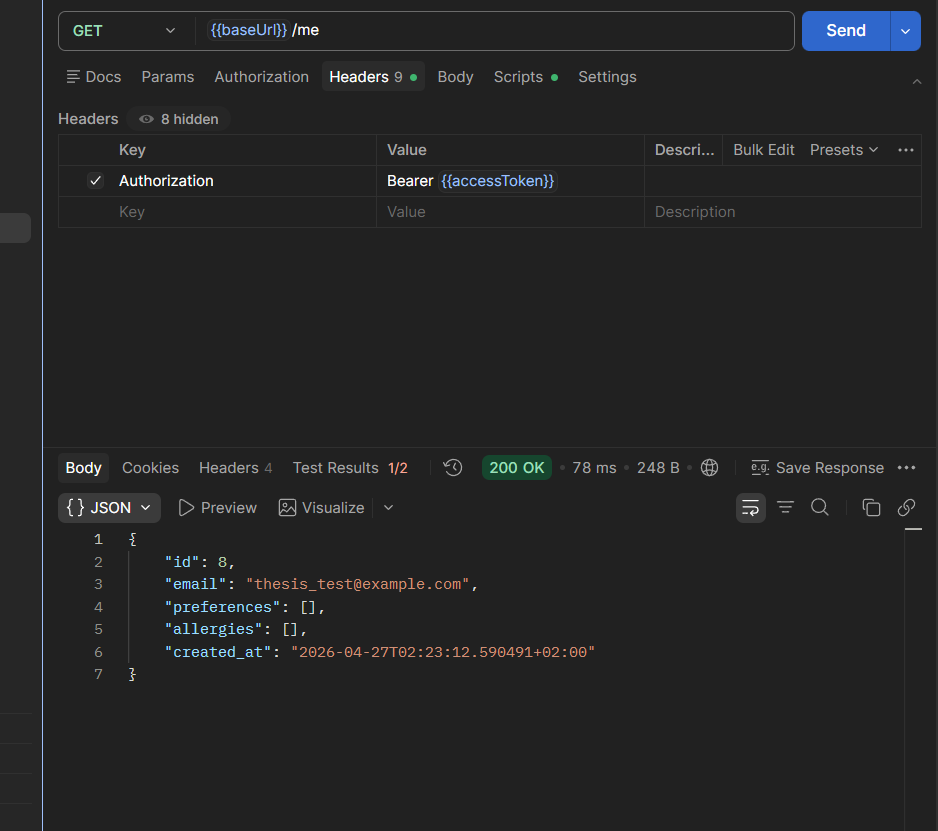
\includegraphics[width=\textwidth]{images/POSTMAN/AuthenticatedProfileRequest.png}
		\caption*{(a) Authenticated \texttt{/me} request}
	\end{minipage}\hfill
	\begin{minipage}{0.48\textwidth}
		\centering
		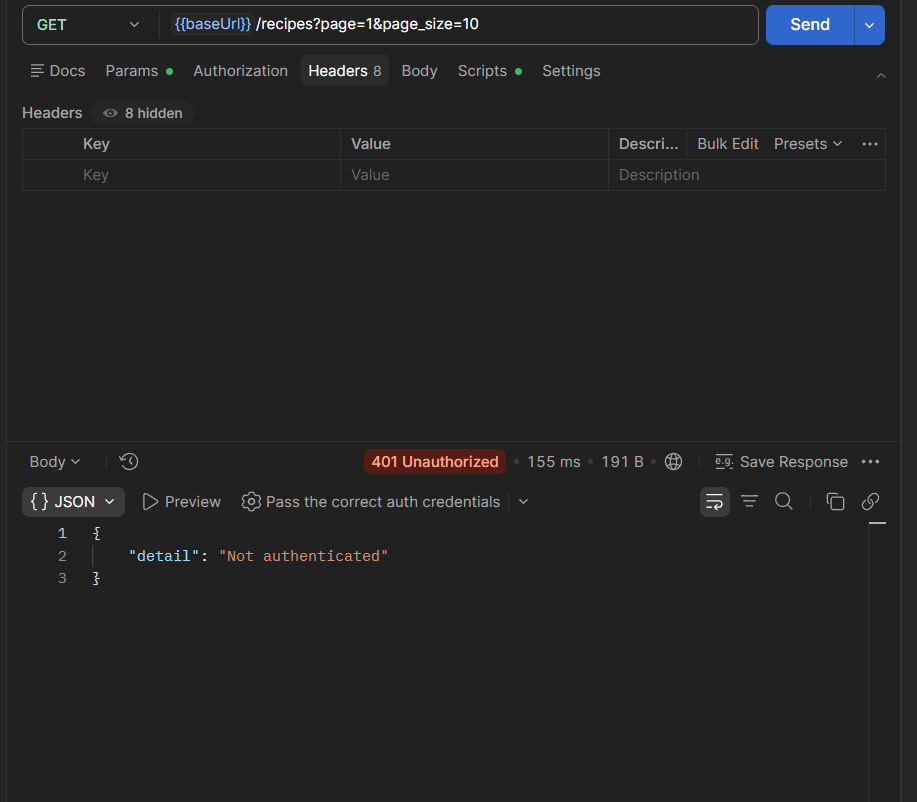
\includegraphics[width=\textwidth]{images/POSTMAN/UnauthorizedProtectedRequest.png}
		\caption*{(b) Unauthorized protected request}
	\end{minipage}
	\caption{Postman evidence for protected-route behavior}
	\label{fig:postman-protected}
\end{figure}

The main recipe-generation integration path is shown in
Figure~\ref{fig:postman-recipe}. The first request demonstrates
successful structured recipe generation through the API. The second
request demonstrates that a generated recipe can then be saved through a
separate persistence endpoint. The third request demonstrates that the
saved or generated item later appears in recipe history.

\begin{figure}[H]
	\centering
	\begin{minipage}{0.32\textwidth}
		\centering
		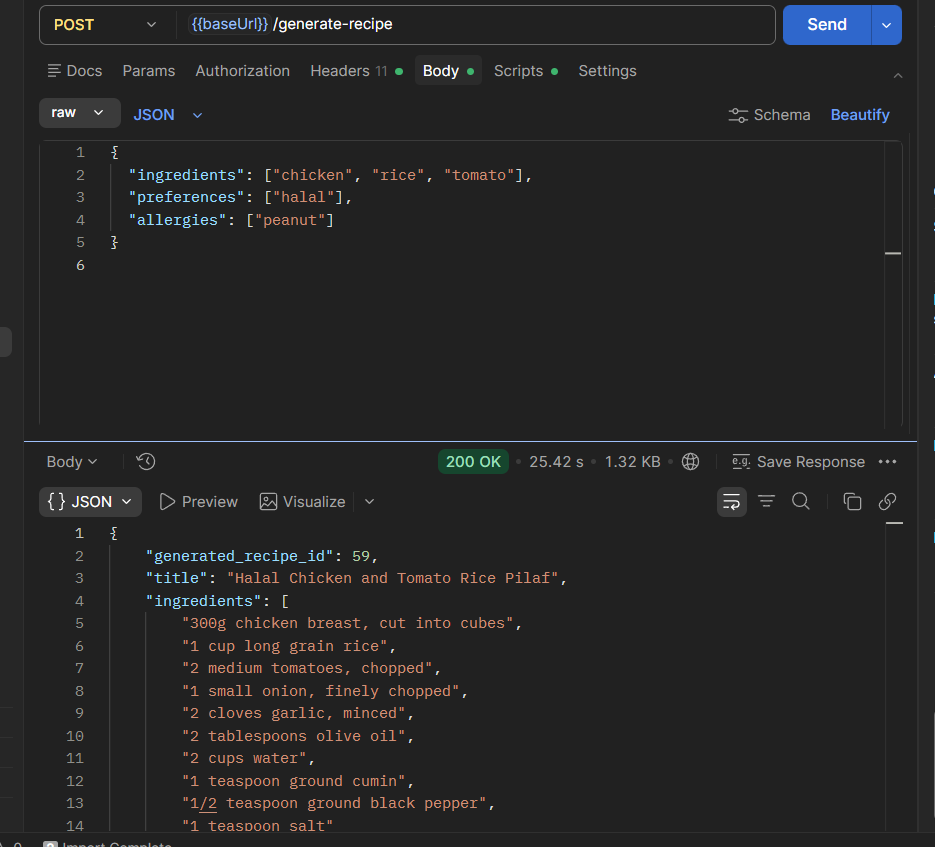
\includegraphics[width=\textwidth]{images/POSTMAN/SuccessfulRecipeGeneration.png}
		\caption*{(a) Recipe generation}
	\end{minipage}\hfill
	\begin{minipage}{0.32\textwidth}
		\centering
		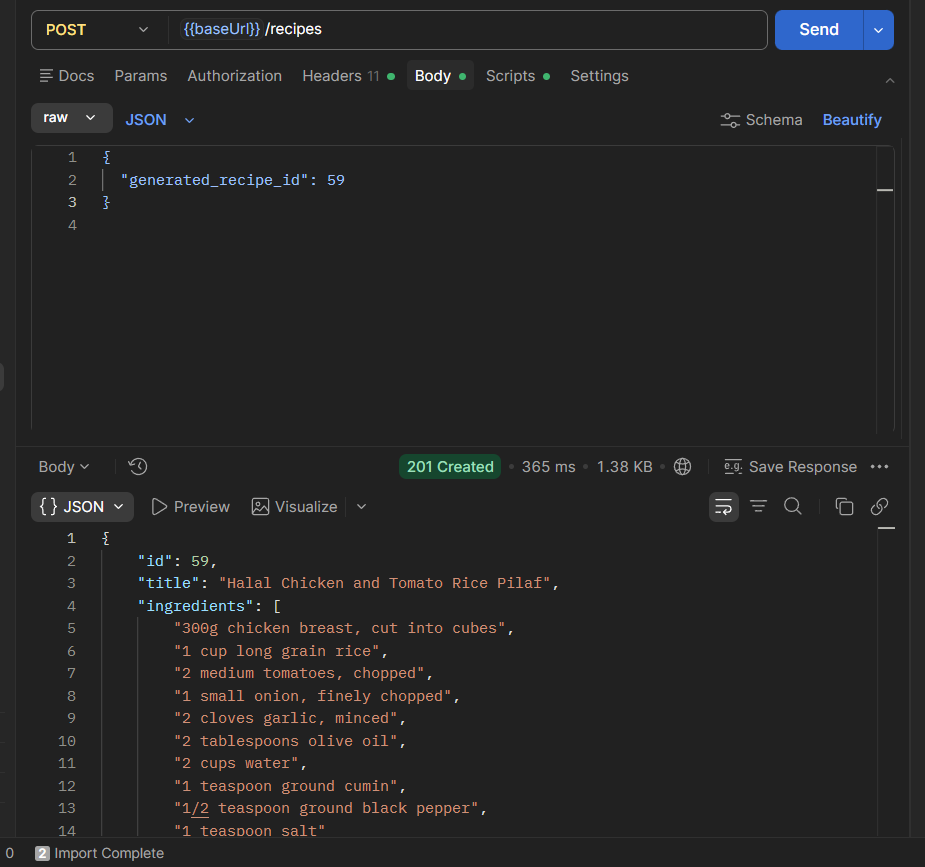
\includegraphics[width=\textwidth]{images/POSTMAN/SaveGeneratedRecipe.png}
		\caption*{(b) Save generated recipe}
	\end{minipage}\hfill
	\begin{minipage}{0.32\textwidth}
		\centering
		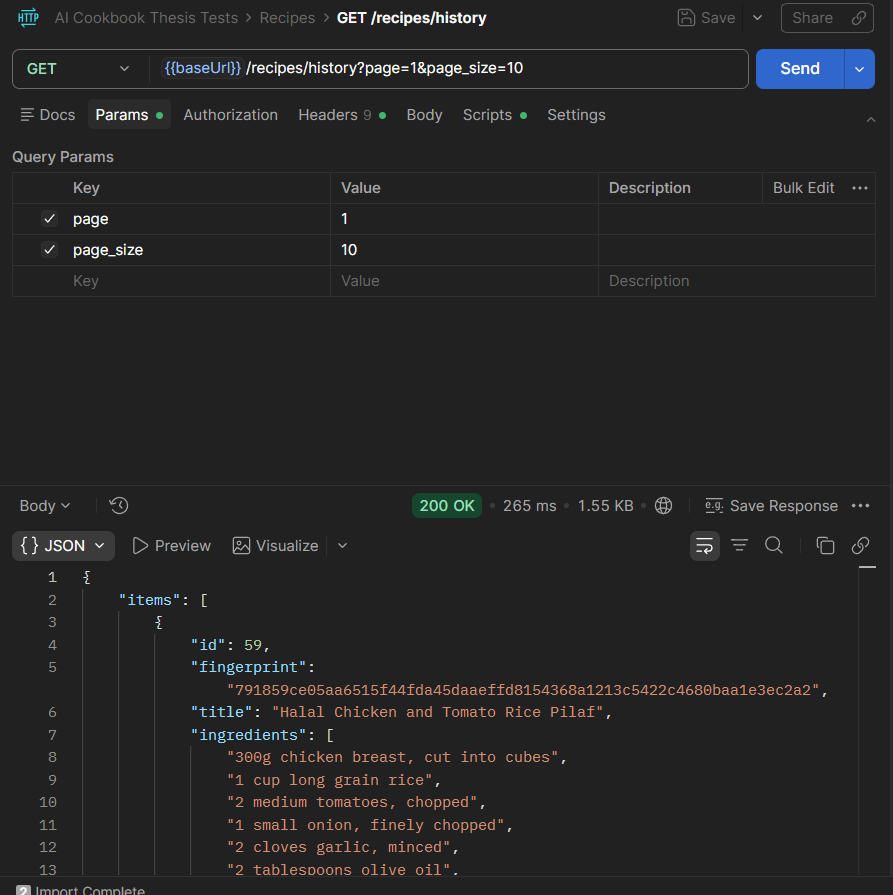
\includegraphics[width=\textwidth]{images/POSTMAN/RecipeHistory.png}
		\caption*{(c) Recipe history retrieval}
	\end{minipage}
	\caption{Postman evidence for recipe-generation and persistence integration}
	\label{fig:postman-recipe}
\end{figure}

This sequence validates a full integration path:

\begin{enumerate}
	\item authenticated user context is accepted,
	\item the recipe-generation endpoint returns structured output,
	\item a generated recipe identifier can be reused by the save endpoint,
	\item the persistence layer stores the record correctly,
	\item the history endpoint returns the stored data through paginated API
	access.
\end{enumerate}

The OCR persistence path is shown in Figure~\ref{fig:postman-ocr}. These
requests confirm that structured OCR-related data can be saved and later
retrieved through the user-scoped history endpoint.

\begin{figure}[H]
	\centering
	\begin{minipage}{0.48\textwidth}
		\centering
		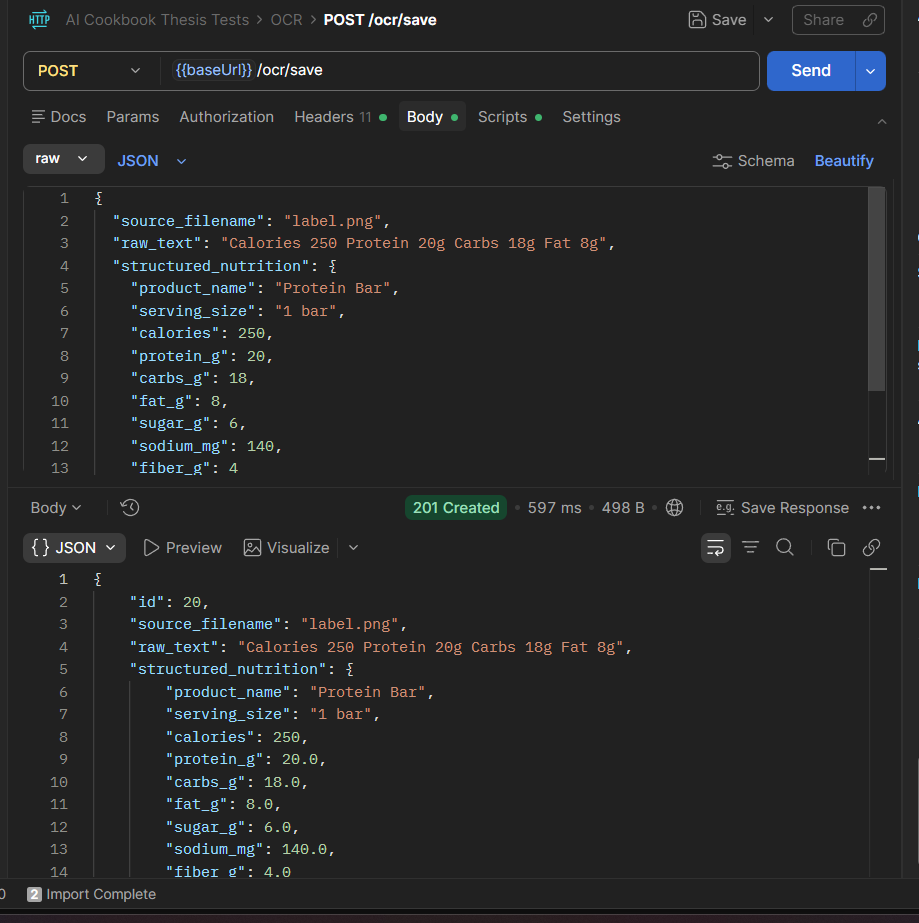
\includegraphics[width=\textwidth]{images/POSTMAN/OCRsave.png}
		\caption*{(a) Save OCR extraction}
	\end{minipage}\hfill
	\begin{minipage}{0.48\textwidth}
		\centering
		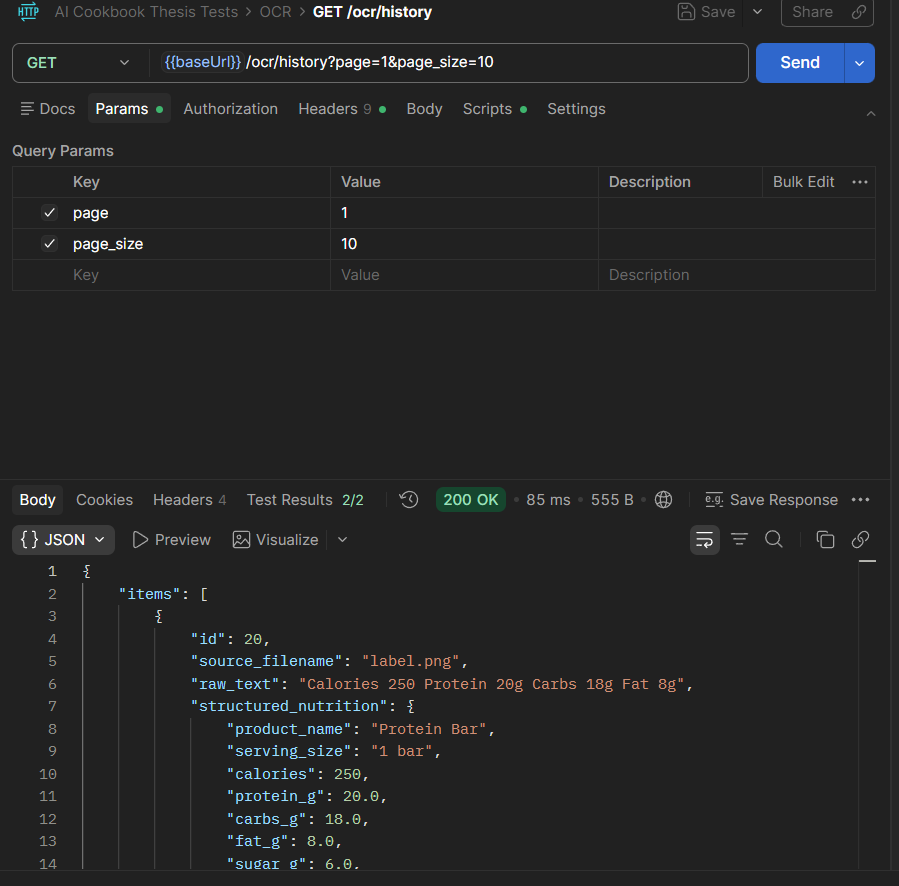
\includegraphics[width=\textwidth]{images/POSTMAN/OCRhistory.png}
		\caption*{(b) OCR history retrieval}
	\end{minipage}
	\caption{Postman evidence for OCR persistence and retrieval}
	\label{fig:postman-ocr}
\end{figure}

Finally, the retrieval subsystem itself is represented by the collection
statistics endpoint shown in Figure~\ref{fig:postman-rag-stats}. This
does not test recipe quality directly, but it does verify that the RAG
layer is implemented as a real subsystem with a persistent collection
and explicit configuration parameters.

\begin{figure}[H]
	\centering
	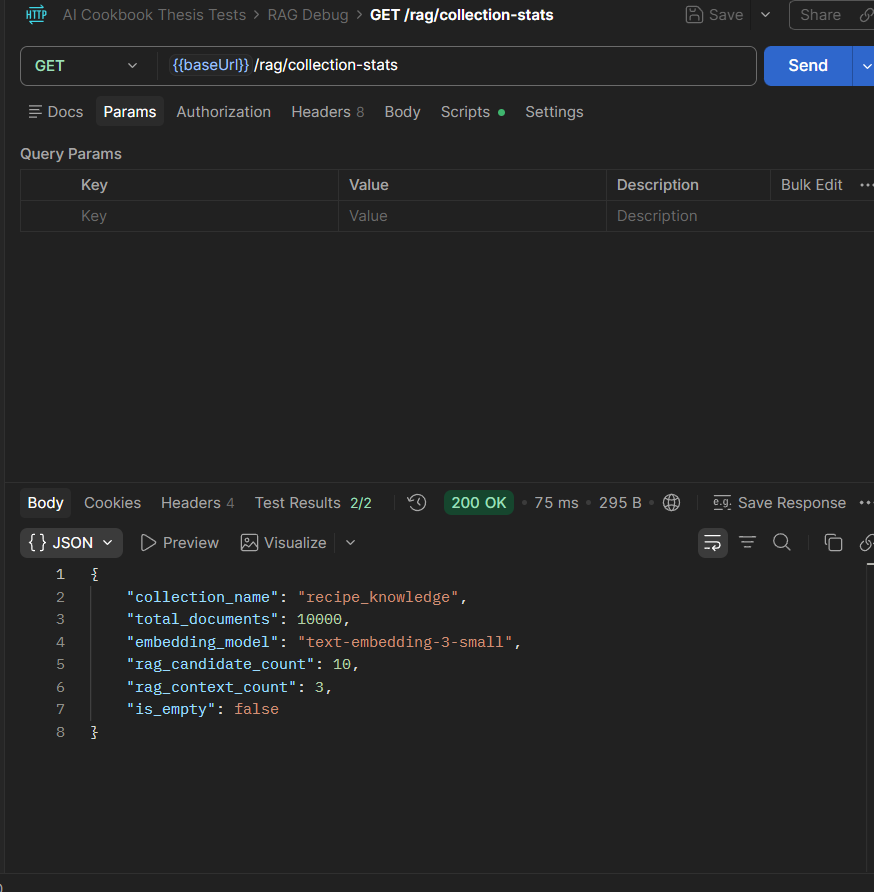
\includegraphics[width=0.78\textwidth]{images/POSTMAN/RAGstats.png}
	\caption{Postman evidence for the retrieval collection statistics endpoint}
	\label{fig:postman-rag-stats}
\end{figure}

Taken together, the Postman evidence validates not just isolated routes,
but real backend integration across authentication, persistence, and
feature-specific workflow boundaries.

\subsection{Advanced Reliability Testing}

\subsubsection{Reliability-oriented backend verification}

In addition to correctness and integration, the backend was also
verified from a reliability perspective. The implemented reliability
tests focus on repeated requests and a small concurrent burst against
the recipe-generation endpoint while external providers are replaced by
deterministic mocks. This approach is appropriate because the project
depends on networked AI services. If those calls were left real during
reliability testing, the results would be dominated by provider latency
and availability rather than the stability of the local application.

The executed reliability-oriented test result is shown in
Figure~\ref{fig:reliability-suite}. The successful run confirms that
the backend can process multiple repeated mocked recipe-generation
requests consistently and can tolerate a small concurrent burst without
failing the internal request path.

\begin{figure}[H]
	\centering
	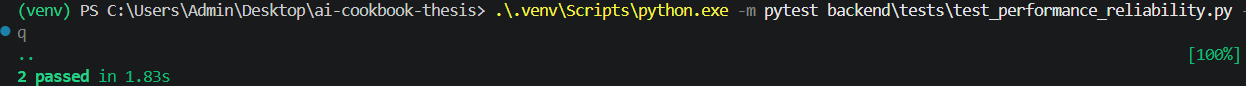
\includegraphics[width=0.9\textwidth]{images/ReliabilityScreenshot.png}
	\caption{Successful reliability-oriented backend test execution}
	\label{fig:reliability-suite}
\end{figure}

This reliability layer should be interpreted carefully. It does
\emph{not} prove real-world latency guarantees for OpenAI or OCR
providers, and it does not replace production load testing. What it
does show is that the internal orchestration of validation, request
handling, and persistence remains stable when the nondeterministic
external dependencies are controlled.

\subsubsection{Role of security-oriented checks}

Security-oriented behavior also appears in the automated and integration
tests. The unauthorized protected-request screenshot in
Figure~\ref{fig:postman-protected} and the backend authentication tests
jointly verify that protected resources are not exposed without a valid
token. The backend rate-limiting tests also validate that repeated
authentication attempts can be restricted at middleware level. For a
project of this scope, this is a meaningful security-oriented testing
layer because it addresses the most relevant risks in the implemented
deployment model: unauthorized access to user-specific saved content and
abusive repeated requests against sensitive endpoints.

\subsection{Manual Scenario-Based Testing}

\subsubsection{Role of manual testing}

Automated backend and frontend tests already confirm a large part of the
deterministic behavior of the application. However, they do not fully
replace scenario-based validation from the perspective of a human user.
Manual testing remains necessary because the project contains
multi-screen workflows that combine authentication state, page
navigation, persistence, generated output display, and OCR result
presentation. These aspects are easier to evaluate coherently when the
system is used as an end user would use it.

For this reason, the project includes a dedicated manual test pack in
\texttt{docs/manual-test-cases.md}. The executed manual cases cover the
main user-facing flows of the application rather than only isolated
controls. The goal of this layer is to confirm that the implemented
features can be completed successfully as end-to-end user tasks and to
support the thesis with screenshot-based evidence.

\subsubsection{Executed manual cases}

The currently executed manual cases cover authentication, profile
management, recipe generation, recipe persistence, history access, OCR
extraction, OCR persistence, and access control. The strongest executed
cases are summarized in Table~\ref{tab:manual-cases-summary}. The table
follows a compact thesis-oriented format similar to classical manual
test documentation: each row identifies the test type, the validated
behavior, the test steps, the expected result, and the observed result.

\begin{table}[H]
	\centering
	\scriptsize
	\renewcommand{\arraystretch}{1.2}
	\begin{tabularx}{\textwidth}{|p{2.2cm}|p{2.0cm}|>{\raggedright\arraybackslash}X|>{\raggedright\arraybackslash}X|>{\raggedright\arraybackslash}X|}
		\hline
		\textbf{Type} & \textbf{Description} & \textbf{Test Steps} & \textbf{Expected Result} & \textbf{Observed Result} \\
		\hline
		\makecell[tl]{UI\\Scenario} & Login page access & Open the frontend, navigate to the Login page, and observe the visible controls. & Login and sign-up tabs are visible, email and password fields are displayed, and the page loads correctly. & The login page loaded successfully and displayed both authentication modes and the required input fields without rendering failure. \\
		\hline
		Functionality & Successful user registration & Open the Login page, switch to Sign Up, enter a valid new email and password, and submit the form. & The account is created successfully, a success message is shown, and the page returns to login mode. & Registration succeeded with valid credentials and the interface returned to the normal authentication flow. \\
		\hline
		Functionality & Successful login and account view & Enter valid user credentials on the Login page, submit the form, and open the Account page. & The user is authenticated successfully and account/profile information is displayed. & The account page displayed the logged-in profile together with the saved preferences and allergies section. \\
		\hline
		\makecell[tl]{Functionality\\Persistence} & Profile default update & Open the Account page, enter dietary preferences and allergies, submit the update form, then refresh or revisit the page. & The profile update succeeds and the new values remain visible after reload. & Updated preference and allergy values remained visible after saving and page revisit, confirming persistence. \\
		\hline
		\makecell[tl]{Functionality\\AI workflow} & Recipe generation with direct input & Open the Generate page, enter a comma-separated ingredient list, and click Generate Recipe. & A structured recipe is returned with title, ingredients, steps, and nutrition estimate, and the page remains stable. & The page returned a complete recipe card and remained stable during response rendering. \\
		\hline
		\makecell[tl]{Functionality\\Personalization} & Recipe generation using saved defaults & Open the Generate page, enter only ingredients, leave preference and allergy fields empty, and generate the recipe. & The stored profile defaults are applied automatically and the generated output reflects those saved constraints. & The generated output reflected the stored personalization settings even though the optional form fields were left blank. \\
		\hline
		\makecell[tl]{Integration\\Persistence} & Save generated recipe & Generate a recipe while logged in, click Save Recipe, then navigate to the Saved page. & The save operation succeeds and the generated recipe appears in the saved recipes list. & The saved recipes page displayed the same recipe after the save action completed. \\
		\hline
		\makecell[tl]{Integration\\Persistence} & Recipe history availability & Generate one or more recipes, open the History page, and inspect the listed entries. & Generated recipes are listed in history, their state is shown, and stored details can be reviewed. & The history page listed the generated entries correctly and allowed their details to be reviewed. \\
		\hline
		\makecell[tl]{Functionality\\OCR} & OCR extraction with valid nutrition label & Open the Food Labels page, upload a valid nutrition-label image, and submit extraction. & The extraction completes successfully and the page displays both raw OCR text and structured nutrition information. & The OCR workflow returned both readable raw text and the expected nutrition field grid for the uploaded label. \\
		\hline
		\makecell[tl]{Integration\\Persistence} & Save OCR extraction & Perform a successful OCR extraction while logged in, save the result, and review the saved label history. & The extraction is stored successfully and appears in the saved OCR history section. & The stored OCR result was later visible in the user-scoped OCR history view. \\
		\hline
		\makecell[tl]{Authentication\\Security} & Protected pages require login & Log out, open the Saved page, then open the History page and observe both responses. & The pages instruct the user to log in and no private saved or historical data is exposed. & Both pages remained inaccessible without authentication and did not expose user-specific content. \\
		\hline
		\makecell[tl]{UI\\Usability} & Expand and collapse saved recipe details & Open the Saved page, expand one saved recipe, then collapse the detail section again. & Steps and nutrition become visible when expanded and are hidden again when collapsed. & The detail section opened and closed correctly while preserving the surrounding page state. \\
		\hline
		\end{tabularx}
	\caption{Manual test cases executed for the AI Cookbook application}
	\label{tab:manual-cases-summary}
\end{table}

The executed manual results show that the application behaves correctly
as a complete user-facing system. Registration and login work in
combination with the account page. Stored preferences and allergies are
reused during recipe generation. Generated recipes can be persisted and
reviewed in the saved-recipes and history views. OCR extraction results
can be produced, saved, and reviewed from history. Protected pages
remain restricted when no authenticated user context is present.

\subsubsection{Relationship to UI and integration testing}

The manual testing layer complements the earlier UI and Postman
sections. UI testing focuses on visible page states and layout-level
evidence. Postman testing focuses on API contracts and HTTP-level
integration. Manual testing documents that a user can complete the full
workflow successfully in the running application.

\subsection{Advanced AI-Related Evaluation}

In addition to deterministic correctness and workflow validation, the
project also includes evaluation of AI-assisted output quality. The
repository therefore contains an evaluation pack for recipe generation
and OCR-based nutrition extraction.

\subsubsection{Recipe-generation evaluation methodology}

The recipe-generation evaluation focuses on the combined behavior of the
RAG retrieval layer, the prompt-driven language-model response, the
restriction-handling logic, and the final structured output returned to
the user. The prepared evaluation cases cover baseline success,
preference satisfaction, allergy filtering, failure handling, and
ingredient drift. Each output was assessed using the following criteria:

\begin{itemize}
	\item \textbf{Structure validity:} whether title, ingredients, steps,
	and nutrition estimate were all present in usable form.
	\item \textbf{Allergy safety:} whether prohibited ingredients were
	successfully excluded or avoided.
	\item \textbf{Preference satisfaction:} whether the generated recipe
	respected the selected dietary rule.
	\item \textbf{Ingredient coverage:} how well the recipe used the
	provided ingredients as its main basis.
	\item \textbf{Additional ingredient count:} how many non-user
	ingredients had to be introduced beyond the basic pantry-like support.
	\item \textbf{Practical quality:} a manual score from 1 to 5 for overall
	usefulness and coherence.
\end{itemize}

\subsubsection{Executed recipe-evaluation results}

Based on the collected recipe outputs, the currently completed
evaluation covers all twelve prepared recipe cases from the repository
worksheet. Eleven of the twelve cases returned a structured recipe
successfully, while one case --- where all provided ingredients
conflicted with the active vegan and milk-avoidance constraints --- was
correctly rejected by the system before unsafe generation could occur.

The aggregated results are summarized in
Table~\ref{tab:recipe-ai-metrics}.

\begin{table}[H]
	\centering
	\scriptsize
	\renewcommand{\arraystretch}{1.2}
	\begin{tabularx}{\textwidth}{|p{4.2cm}|p{2.6cm}|>{\raggedright\arraybackslash}X|}
		\hline
		\textbf{Metric} & \textbf{Value} & \textbf{Interpretation} \\
		\hline
		Total evaluated recipe cases & 12 & Full prepared recipe set was executed. \\
		\hline
		Successful responses & 11 / 12 & Only the fully conflicting input was rejected. \\
		\hline
		Structure validity rate & 91.7\% & Most cases returned complete structured recipe output. \\
		\hline
		Allergy safety rate & 100\% & Allergy-constrained cases stayed safe or were correctly rejected. \\
		\hline
		Preference satisfaction rate & 100\% & Preference-constrained cases respected the declared rule set. \\
		\hline
		Average ingredient coverage score & 0.75 & Most outputs used the provided ingredients well, though conflict-removal cases naturally reduced coverage. \\
		\hline
		Average additional ingredient count & 0.33 & Extra ingredients were generally limited. \\
		\hline
		Average practical quality score & 4.4 / 5 & The outputs were usually coherent and usable in practice. \\
		\hline
		\end{tabularx}
	\caption{Aggregated metrics for recipe-generation AI evaluation}
	\label{tab:recipe-ai-metrics}
\end{table}

The structure validity rate shows that the model usually returns output
in the required application format. The safety and preference metrics
show that the combination of conflict filtering, restriction-aware
prompting, and post-generation validation was effective in the executed
cases. Lower ingredient-coverage scores were expected in cases where
one of the user-provided ingredients conflicted with an allergy or
dietary preference, because the system favored safety over maximal
ingredient reuse.

\subsubsection{Representative recipe-evaluation observations}

The executed outputs also reveal several meaningful qualitative
patterns.

\begin{itemize}
	\item In baseline cases such as vegetarian pasta or simple salad input,
	the generated recipes remained coherent, simple, and strongly centered
	on the user ingredients.
	\item In allergy-constrained cases such as peanut, milk, and shellfish
	avoidance, the system issued explicit warnings and removed the
	conflicting ingredient while still attempting to preserve recipe
	usability.
	\item In preference-conflict cases such as vegetarian input containing
	chicken, the system again preferred rule compliance over preserving the
	conflicting ingredient.
	\item In some simple-input cases, the system suggested one or two extra
	ingredients, which improved practicality but slightly increased
	ingredient drift.
	\item In the fully conflicting case, the system correctly rejected the
	request instead of generating an unsafe or nonsensical output.
\end{itemize}

These observations show that the surrounding rule logic influences the
final quality and safety of the generated result.

\subsubsection{Executed OCR evaluation results}

The OCR-specific evaluation was executed on three representative images:
a clear nutrition label, a different supplement-style label layout, and
a deliberately invalid non-nutrition document. This evaluation measures
whether OCR text is returned and whether the downstream structuring
stage produces correct nutrition fields or rejects unsuitable input.

Table~\ref{tab:ocr-case-summary} summarizes the per-case outcomes. For
the two valid label images, the system extracted all core numeric
nutrition fields correctly. The third case reveals the current failure
mode: the OCR stage successfully read the document text, but the
nutrition-structuring layer still returned a zero-filled nutrition
object instead of rejecting the non-target image as unsupported input.

\begin{table}[H]
		\centering
		\scriptsize
		\renewcommand{\arraystretch}{1.2}
		\begin{tabularx}{\textwidth}{|p{1.15cm}|>{\raggedright\arraybackslash}X|p{1.4cm}|p{1.8cm}|p{1.8cm}|>{\raggedright\arraybackslash}X|}
			\hline
			\textbf{Case} & \textbf{Input type} & \textbf{OCR success} & \textbf{Structured output} & \textbf{Correct fields} & \textbf{Observation} \\
			\hline
			O-01 & Clear nutrition label (\texttt{nutrition-facts.jpg}) & Yes & Yes & 9 / 9 & Serving size and all numeric nutrition values were extracted correctly from the clean label image. \\
			\hline
		O-02 & Alternate supplement-label layout (\texttt{unnamed.jpg}) & Yes & Yes & 9 / 9 & The different visual layout still produced correct serving-size and nutrition values across the core fields. \\
		\hline
		O-03 & Non-nutrition certificate photo (\texttt{WhatsApp Image 2026-04-14 at 13.56.17.jpeg}) & Yes & No & 0 / 9 & OCR text was extracted from the document, but the nutrition layer should have rejected the image instead of returning zero-valued nutrition fields. \\
		\hline
	\end{tabularx}
	\caption{Executed OCR evaluation cases and outcomes}
	\label{tab:ocr-case-summary}
\end{table}

The aggregate OCR metrics are summarized in
Table~\ref{tab:ocr-ai-metrics}. These values show that the OCR pipeline
is strong on valid label images, but still needs a better front-end
screening or classifier step for non-label uploads.

\begin{table}[H]
	\centering
	\scriptsize
	\renewcommand{\arraystretch}{1.2}
	\begin{tabularx}{\textwidth}{|p{4.2cm}|p{2.4cm}|>{\raggedright\arraybackslash}X|}
		\hline
		\textbf{Metric} & \textbf{Value} & \textbf{Interpretation} \\
		\hline
		Total evaluated OCR cases & 3 & Two valid label images and one invalid non-label document were executed. \\
		\hline
		OCR text extraction success rate & 100\% & Text was extracted from all three images, including the invalid document. \\
		\hline
		Structured-output success rate & 66.7\% & Only the two real nutrition-label images produced semantically correct structured nutrition output. \\
		\hline
		Calories exact-match rate & 66.7\% & Calories were correct for both valid labels and incorrect for the invalid document case. \\
		\hline
		Macro-field exact-match rate & 66.7\% & Protein, carbohydrate, fat, sugar, sodium, and fiber fields were correct on the valid labels and failed on the invalid document. \\
		\hline
		Average correctly extracted fields per image & 6.0 / 9 & The strong valid cases are offset by the complete failure of the non-target document case. \\
		\hline
		High-quality extraction share (\(\geq 5\) correct fields) & 66.7\% & Two of the three evaluated images produced practically useful structured results. \\
		\hline
	\end{tabularx}
	\caption{Aggregated metrics for OCR evaluation}
	\label{tab:ocr-ai-metrics}
\end{table}

These OCR results show that the implemented OCR plus structuring
pipeline works well on clear nutrition labels of more than one visual
layout. They also expose a current limitation: the system needs an
explicit rejection rule or document-type classifier before the
nutrition structuring stage, because raw OCR success alone is not
enough to guarantee semantic correctness.

\subsection{Threats to Validity}

The current testing evidence has several limitations that should be
stated explicitly.

\begin{itemize}
	\item External AI providers can change behavior over time, so backend
	correctness does not imply identical future qualitative outputs.
	\item The reliability tests use mocked dependencies and therefore do not
	measure real-world latency of OpenAI or OCR services.
	\item Screenshot-based UI verification demonstrates usability and
	correct rendering, but it is not a substitute for exhaustive browser
	automation across all edge cases.
	\item The manual scenario evidence is strong for the main workflows,
	but it still prioritizes representative end-user tasks over exhaustive
	permutation of every negative and pagination edge case.
	\item The OCR evaluation currently uses only three executed images, so
	its metrics already reveal meaningful behavior, but they should still
	be interpreted as a small-sample evaluation rather than a production-
	scale benchmark.
\end{itemize}

These limitations define the interpretation boundary of the evidence
presented in this chapter.

\subsection{Chapter Summary}

The testing evidence consists of multiple complementary layers.
Automated backend tests verified authentication, persistence,
validation, retrieval support logic, and OCR-related services.
Automated frontend tests verified page behavior and conditional
rendering. Screenshot-based UI verification documented the implemented
user workflows. Postman-based integration checks verified API behavior,
token-based authentication, persistence endpoints, recipe history, OCR
history, and retrieval statistics across component boundaries.
Reliability-oriented backend tests showed stable local request handling
under repeated mocked requests and small bursts. Coverage measurement
showed that the automated suites exercised a large part of the
implemented backend and frontend logic, especially the
security-sensitive and user-visible layers. Manual scenario-based
testing confirmed that the main end-user workflows can be completed in
the running application. AI-specific evaluation showed that recipe
generation performed well across the prepared worksheet and that OCR
worked well on valid labels while still exposing a meaningful failure
mode on non-nutrition input.

The chapter therefore documents both the functional correctness of the
implemented system and the current quality boundary of its AI-assisted
features.
